%
% $Id: $
%
%
% Compilar a .pdf con LaTeX (pdflatex)
% Es necesario instalar Beamer (paquete latex-beamer en Debian)
%

%
% Gráficos:
% Los gráficos pueden suministrarse en PNG, JPG, TIF, PDF, MPS
% Los EPS deben convertirse a PDF (usar epstopdf)
%

\documentclass{beamer}
\usetheme{Warsaw}
\usebackgroundtemplate{
\includegraphics[width=\paperwidth]{format/libresoft-bg-soft.png}}
\usepackage[spanish]{babel}
\usepackage[utf8]{inputenc}
\usepackage{graphics}
\usepackage{amssymb} % Simbolos matematicos

%\definecolor{libresoftgreen}{RGB}{162,190,43}
%\definecolor{libresoftblue}{RGB}{0,98,143}

%\setbeamercolor{titlelike}{bg=libresoftgreen}

%% Metadatos del PDF.
\hypersetup{
  pdftitle={Communities / Master on Libre Software (URJC)},
  pdfauthor={Felipe Ortega},
  pdfcreator={GSyC/LibreSoft, Universidad Rey Juan Carlos},
  pdfproducer=PDFLaTeX,
  pdfsubject={},
}
%%

% \includeonly{data-mining}
\includeonly{linear-models-R}

\AtBeginSection[]
{
\begin{frame}<beamer>
\begin{center}
{\Huge \insertsection}
\end{center}
\end{frame}
}

\begin{document}

\title{Communities}
\subtitle{Master on Libre Software (URJC) \\
\url{http://master.libresoft.es}}
\author{Felipe Ortega}
\institute{jfelipe@libresoft.es\\
@jfelipe
GSyC/LibreSoft, Universidad Rey Juan Carlos}

\date{February 2011}

\frame{
\maketitle
\begin{center}

\includegraphics[width=6cm]{format/gsyc-urjc}
\end{center}
}


% Si el titulo o el autor se quieren acortar para los pies de página
% se pueden redefinir aquí:
%\title{Titulo corto}
%\author{Autores abreviado}


%% LICENCIA DE REDISTRIBUCION DE LAS TRANSPAS
\frame{
~
\vspace{3cm}

\begin{flushright}
{\tiny \copyright 2011 Felipe Ortega. \\

Some rights reserved. \\
This document is distributed under the \\
Creative Commons Attribution-ShareAlike 3.0 licence, \\
available in \\
\url{http://creativecommons.org/licenses/by-sa/3.0}

The original version of this document is available at \\
\url{http://master.libresoft.es}
}
\end{flushright}
}
% Slides

%% introduction.tex
%%
%% Introduction to the course ``Economic aspects'' of the
%%   Official Master on Libre Software (URJC)
%%   http://master.libresoft.es

%%---------------------------------------------------------------------
%%---------------------------------------------------------------------
\section{Introduction to data mining}

%%---------------------------------------------------------------------
\subsection{What is data mining?}

%%---------------------------------------------------------------

\begin{frame}
\frametitle{Data explosion in the digital age}

\begin{itemize}
 \item Massive, ever-growing, digital datasets.
 \item Spread of open datasets.
 \begin{itemize}
  \item FLOSS projects (version control, issue tracking, mailing lists...)
  \item Social media (Twitter, Identi.ca...)
  \item WWW (web pages, blogs, photo sites, content tagging, news sites...)
  \item Compilations (Internet archive, Wikimedia Commons, Creative Commons...)
  \item Open government (laws and policies, archives and records, budgets...)
 \end{itemize}

\end{itemize}

\begin{flushright}
``We are data rich, but information poor'' \\
{\small [Han and Kamber, 2006]}
\end{flushright}
\end{frame}

%%---------------------------------------------------------------

\begin{frame}
\frametitle{A definition for data mining}

\begin{quote}
 ``Extracting or mining knowledge from large amounts of data''
\end{quote}
\begin{flushright}
{\small [Han and Kamber, 2006]}
\end{flushright}

\begin{quote}
 ``The \textit{non-trivial }extraction of \textit{implicit}, previously unknown, and potentially
useful information from data''.
\end{quote}
\begin{flushright}
{\small [Frawley et al., 1991]}
\end{flushright}


\end{frame}

%%---------------------------------------------------------------

\begin{frame}
\frametitle{Do not confuse data mining with...}

\begin{itemize}
 \item Data warehouse: Information repository integrated from different
sources, organized under a common schema and usually stored in a sigle location.

 \item Data mart: Subset of a data warehouse, spanning a single department.

 \item On-Line Analytical Processing (OLAP): Summarization techniques allowing us
to inspect a data warehouse from multiple perspectives, at different abstraction levels.

\end{itemize}

\end{frame}

%%---------------------------------------------------------------

\begin{frame}
\frametitle{Do not confuse data mining with...}

\begin{itemize}

 \item Statistical analysis: Application of statistical tools and techniques (part of the data
mining process) to describe and
summarize datasets, as well as to create models suitable for interpreting and understanding 
reality from these datasets.

 \item Machine learning: Automated tools and techniques (part of the data mining process) 
that we can use to identify hidden patterns in data. They usually involve an initial training phase.

\end{itemize}

\end{frame}

%%---------------------------------------------------------------

\begin{frame}
\frametitle{Stages in data mining}

Origin: data sources/datasets

\begin{enumerate}
 \item Identification of data sources.
 \item Data selection/sampling.
 \item Data preparation.
 \item Data transformation.
 \item Model building.
 \item Model evaluation.
 \item Visualization and presentation of results.
\end{enumerate}

Goal: Knowledge discovery (\textit{models} or \textit{patterns}).

\begin{flushright}
{\small [Nisbet et al., 2009]}
\end{flushright}

\end{frame}

%%---------------------------------------------------------------

\begin{frame}
\frametitle{Data Mining tasks}

\begin{itemize}
 \item Description.
 \item Estimation.
 \item Prediction.
 \item Classification.
 \item Clustering.
 \item Association.
\end{itemize}

\begin{flushright}
{\small [Larose, 2005]}
\end{flushright}

\end{frame}

%%---------------------------------------------------------------------
\subsection{A quick tour through data mining techniques}

%%---------------------------------------------------------------

\begin{frame}
\frametitle{Data preparation for data mining}

\begin{itemize}
 \item Oftenly disregarded, but \textbf{essential} for success.
 \item Understanding collected data.
 \item Data model, data types...
 \item Storage platform.
 \item Special attention to \textbf{missing values}.
 \begin{itemize}
  \item Imputation techniques (statistics).
 \end{itemize}
 \item Sampling, transformation, series variables.
 \item Categorical variables (R factors).
\end{itemize}


\end{frame}

%%---------------------------------------------------------------

\begin{frame}
\frametitle{Exploratory Data Analysis (EDA)}

\begin{itemize}
 \item Data summarization.
 \item Summary statistics.
 \item Time plot, scatter plot.
 \item Histogram, density estimation.
 \item Boxplot.

\end{itemize}

\end{frame}

%%---------------------------------------------------------------

\begin{frame}
\frametitle{Exploratory Data Analysis (EDA)}

\begin{center}
 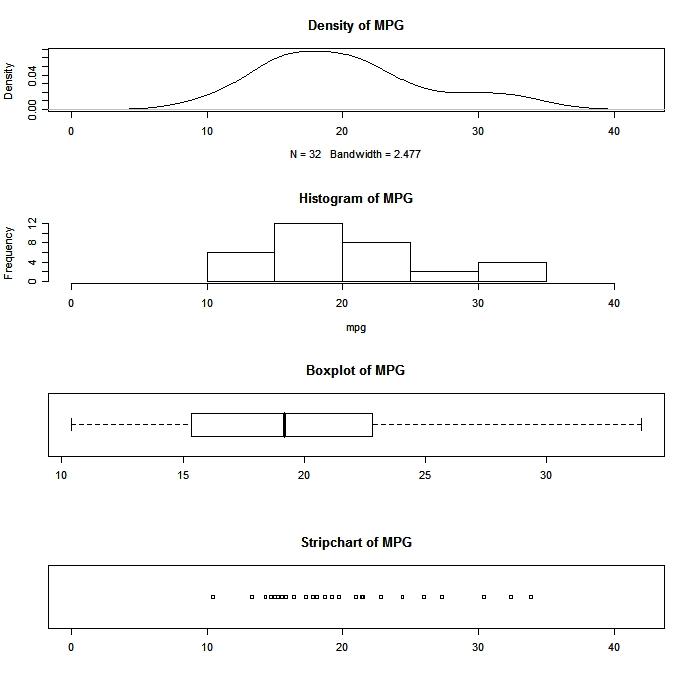
\includegraphics[height=6cm]{figs/simpleplots.jpg}
\end{center}

\begin{flushright}
\small Examples with GNU R.
\end{flushright}

\end{frame}

%%---------------------------------------------------------------

\begin{frame}
\frametitle{Classification: pattern recognition}

Problem: Identification of patterns, groups, taxonomies hidden in
data. Outputs: Label assigned to inputs based on a certain algorithm.

\begin{center}
 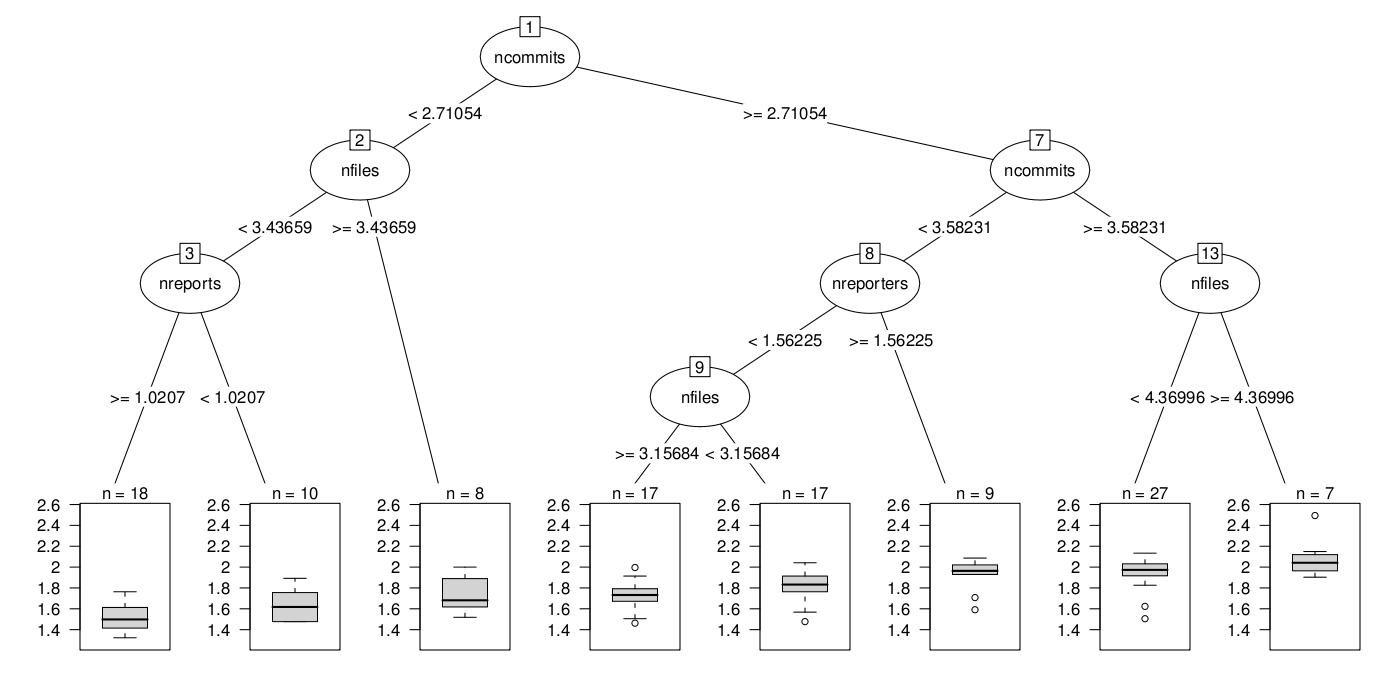
\includegraphics[height=4.5cm]{figs/tree-projects.jpg}
\end{center}

\begin{flushright}
\small Classification tree Flossmetrics projects.
\end{flushright}

\end{frame}

%%---------------------------------------------------------------

\begin{frame}
\frametitle{Prediction: statistical models}

The goal is to create a model based on a set of inputs (explanatory variables) to characterize
the behaviour of a output (response variable).

\begin{itemize}
 \item Linear models (regression...).
 \item Generalized linear models (GLM).
 \item Non-linear models.
 \item Multilevel models (response varies at more than one level).
\end{itemize}


\end{frame}

%%---------------------------------------------------------------

\begin{frame}
\frametitle{Prediction: statistical models}

\begin{center}
 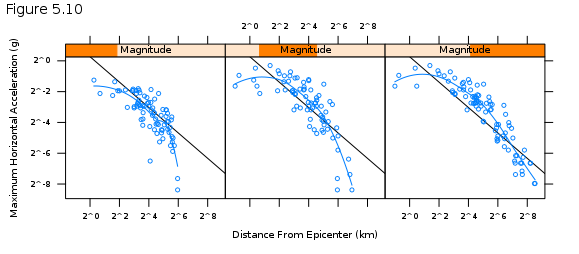
\includegraphics[height=4.5cm]{figs/linear-models.png}
\end{center}

\begin{flushright}
\small Example: fitting linear models (lattice).
\end{flushright}

\end{frame}

%%---------------------------------------------------------------

\begin{frame}
\frametitle{Cluster analysis}

\begin{itemize}
 \item Goal: identification of ``clusters'' of related data points.
 \item Many different algorithms:
 \begin{itemize}
  \item Partitioning methods: k-means, k-mediods.
  \item Hierarchical methods: agglomerative vs. divisive.
  \item Density based methods.
  \item Grid-based methods.
  \item Model-based methods.
  \item Clustering high-dimensional data.
 \end{itemize}

\end{itemize}

\end{frame}

%%---------------------------------------------------------------

\begin{frame}
\frametitle{Cluster analysis}

\begin{center}
 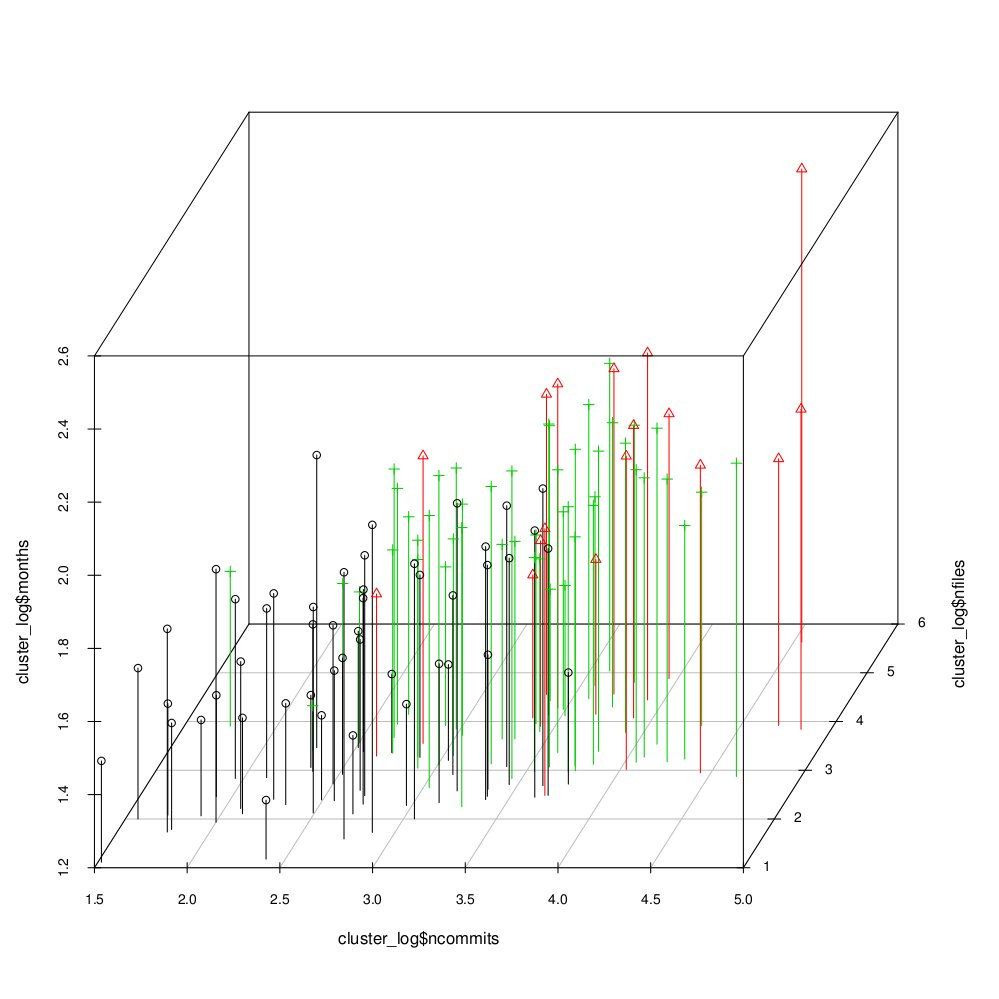
\includegraphics[height=6cm]{figs/cluster3D.jpg}
\end{center}

\begin{flushright}
\small Clustering Flossmetrics projects.
\end{flushright}

\end{frame}

%%---------------------------------------------------------------

\begin{frame}
\frametitle{Streams, time-series and sequential data}

\begin{itemize}
 \item Longitudinal analysis (statistics).
 \item Time always introduces particular conditions in the analysis.
 \item Time-sereis analysis, trends, forecasting.
 \item ARMA, ARIMA models.
\end{itemize}


\end{frame}

%%---------------------------------------------------------------

\begin{frame}
\frametitle{Streams, time-series and sequential data}

\begin{center}
 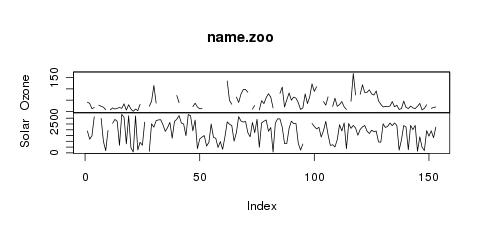
\includegraphics[height=4.5cm]{figs/timeseries.jpg}
\end{center}

\begin{flushright}
\small Example of irregular timeseries [Kukuyeva, 2010].
\end{flushright}

\end{frame}

%%---------------------------------------------------------------

\begin{frame}
\frametitle{Graph mining, Social Network Analysis}

\begin{itemize}
 \item Goal: Study network of nodes, properties, evolution over time.
 \item Web graph, social graph.
 \item Many properties: degree centrality, hubs and authorities, betweeness, transitivity, reciprocity...
 \item Powerful R packages: sna, igraph, statnet.
\end{itemize}

\begin{flushright}
\small [Newman, 2010], [Conway, 2009]
\end{flushright}

\end{frame}

%%---------------------------------------------------------------

\begin{frame}
\frametitle{SNA in R (I)}

\begin{center}
 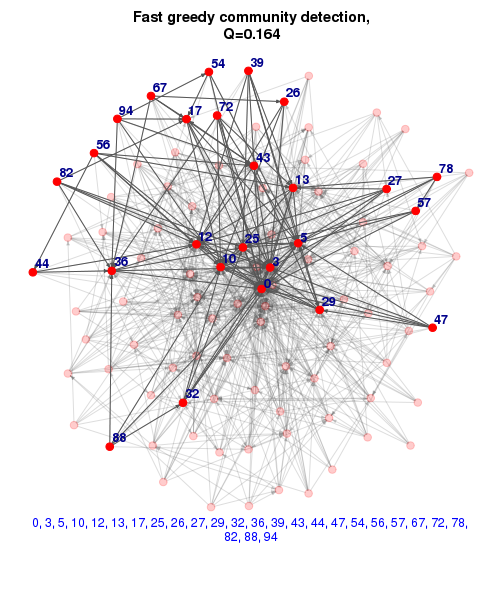
\includegraphics[height=5.5cm]{figs/sna1-igraph.png}
\end{center}

\begin{flushright}
\small Transparencies in network graphs (R igraph).
\end{flushright}

\end{frame}

%%---------------------------------------------------------------

\begin{frame}
\frametitle{SNA in R (II)}

\begin{center}
 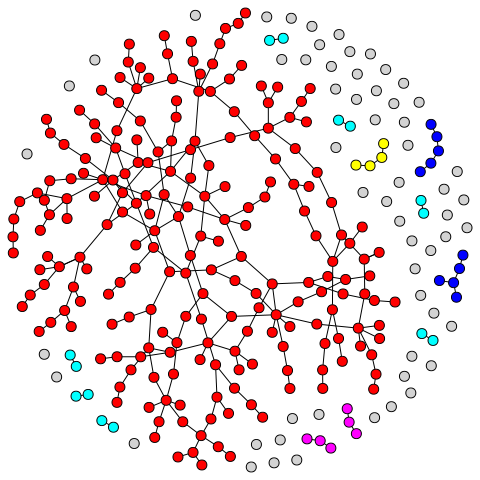
\includegraphics[height=5.5cm]{figs/sna2-igraph.png}
\end{center}

\begin{flushright}
\small Coloured nodes (R igraph).
\end{flushright}

\end{frame}

%%---------------------------------------------------------------

\begin{frame}
\frametitle{SNA in R (III)}

\begin{center}
 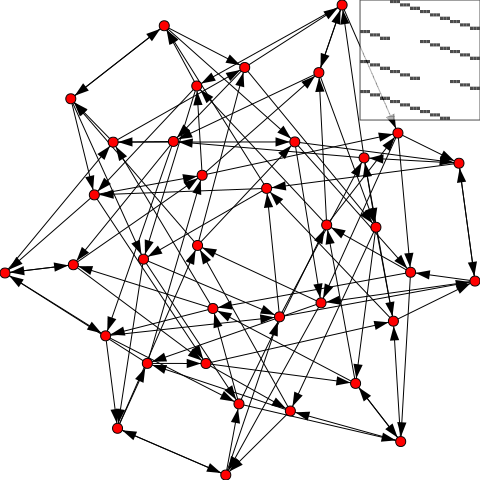
\includegraphics[height=5.5cm]{figs/sna3-igraph.png}
\end{center}

\begin{flushright}
\small Directed networks (R igraph).
\end{flushright}

\end{frame}

%%---------------------------------------------------------------

\begin{frame}
\frametitle{Mining special types of data}

\begin{itemize}
 \item Spatial data.
 \item Multimedia data.
 \item Text mining.
 \item Structured web data.
\end{itemize}


\end{frame}

%%---------------------------------------------------------------------
\subsection{The last step: visualization and reports}

%%---------------------------------------------------------------

\begin{frame}
\frametitle{Visualization tools}

\begin{itemize}
 \item Specialized R packages:
 \begin{itemize}
  \item lattice.
  \item ggplot2.
  \item rggobi
 \end{itemize}

\end{itemize}

\end{frame}

%%---------------------------------------------------------------

\begin{frame}
\frametitle{Visualization tools}

\begin{itemize}
 \item Processing: powerful framework for visualization and design
 \begin{itemize}
  \item Affordable learning curve.
  \item More flexibility with Processing.js (JavaScript port).
  \item Example: \url{http://mattmckeon.com/facebook-privacy/}
 \end{itemize}

\end{itemize}

\end{frame}

%%---------------------------------------------------------------

\begin{frame}
\frametitle{Visualization tools}

\begin{itemize}
 \item Crowdsourcing options.
 \begin{itemize}
  \item Many Eyes: \url{http://www-958.ibm.com/software/data/cognos/manyeyes/}
 \end{itemize}

\end{itemize}

\end{frame}

%%---------------------------------------------------------------

\begin{frame}
\frametitle{Rapid Miner}

\begin{itemize}
 \item Integrated, libre software, data mining suite.
 \item Conceived for interactive users.
 \item Many useful extensions: R connection, paralelization, time series...
 \begin{itemize}
  \item Website: \url{http://rapid-i.com/}
 \end{itemize}

\end{itemize}

\end{frame}

%%---------------------------------------------------------------

\begin{frame}
\frametitle{Rapid Miner}

\begin{center}
 \begin{LARGE} LIVE DEMO \end{LARGE}
\end{center}


\end{frame}


%%---------------------------------------------------------------

% \begin{frame}
% \frametitle{The growth of libre software (2)}
% 
% 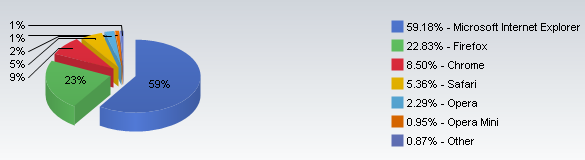
\includegraphics[height=3.5cm]{webbrowsers-share-2010-10}
% 
% \begin{flushright}
% Net Market Share Report, October 2010 \\
% {\small \url{http://www.netmarketshare.com/}}
% \end{flushright}
% \end{frame}

%%---------------------------------------------------------------------
\subsection{References}

%%---------------------------------------------------------------

\begin{frame}
\frametitle{References on data mining}

\begin{itemize}
 \item \small [Han and Kamber, 2006] Han, J. and Kamber, M. (2006). Data Mining: Concepts and Techniques (2nd ed.). 
 San Francisco: Morgan Kaufmann.
 \item \small [Frawley et al., 1991] Frawley, W., Piatetsky-Shapiro, G., and Matheus, C. (1991). Knowledge discovery 
in databases—An overview. In Knowledge Discovery in Databases 1991 (pp. 1–30). Reprinted in AI Magazine, Fall 1992.
 \item \small [Nisbet et al., 2009] Nisbet, R., Elder, J. and Miner, G. (2009). Handbook of Statistical Analyses and
Data Mining Applications. Academic Press.
 \item \small [Larose, 2005] Larose, D. T. (2005). Discoverying Knowledge in Data: An Introduction to Data Mining.
John Wiley \& Sons.

 \end{itemize}
\end{frame}

%%---------------------------------------------------------------

\begin{frame}
\frametitle{References on useful techniques}

\begin{itemize}
 \item \small [Newman, 2010] Newman, M. E. J. (2010). Networks: An introduction. Oxford University Press.
 \item \small [Wasserman and Faust, 1994] Wasserman, S. and Faust, K. (1994). Social Network Analysis.
Cambridge University Press.
 \item \small [Xu, Wunsch 2008] Xu, R. and Wunsch, D. (2008). Clustering. Wiley-IEEE Press.
 \item \small [Witten et al., 2011] Witten, I. H., Frank, E. and Hall, M. A. (2011). Data Mining: Practical Machine 
Learning Tools and Techniques, Third Edition. Morgan Kaufmann.

 \end{itemize}
\end{frame}

%%---------------------------------------------------------------

\begin{frame}
\frametitle{Presentations and tutorials (GNU R)}

\begin{itemize}
 \item \small [Kukuyeva, 2010] Kukuyeva, I. Intermediate Graphics with R.
 \url{http://scc.stat.ucla.edu/page_attachments/0000/0120/10w-int-graphics.zip}
 \item \small [Conway, 2009] Conway, D. Social Network Analysis in R.
 \url{http://www.drewconway.com/zia/?p=1221}
 \item \small [Rosario, 2010] Rosario, R. Advanced Graphics in R.
 \url{http://www.bytemining.com/?p=34}
 \item R-bloggers: \url{http://www.r-bloggers.com/}

 \end{itemize}
\end{frame}

%%---------------------------------------------------------------

%% introduction.tex
%%
%% Introduction to the course ``Economic aspects'' of the
%%   Official Master on Libre Software (URJC)
%%   http://master.libresoft.es

%%---------------------------------------------------------------------
%%---------------------------------------------------------------------
\section{Linear models in R}

%%---------------------------------------------------------------

\begin{frame}
\frametitle{Linear models}

The goal is to fit a model characterizing the behavior of an \textbf{output} (response or dependant)
variable, according to one or several \textbf{input} (predictor, independent or explanatory) variables.

\end{frame}

%%---------------------------------------------------------------

\begin{frame}
\frametitle{Preparing your linear model}

\begin{itemize}
  \item Identify your response variable
  \item Identify the explanatory variable(s).
  \item Are the explanatory variables continuous, factors (categorical) or mixed?
  \item What's the type of your response variable (continuous, factor, count, proportion, binary, time at death, category)
\end{itemize}

\end{frame}

%%---------------------------------------------------------------

\begin{frame}
\frametitle{Available linear models}
\textbf{Explanatory variables}
\begin{itemize}
\item All continuous: Regression.
\item All categorical: Analysis of Variance (ANOVA).
\item Mixed: Analysis of Covariance (ANCOVA).
\end{itemize}

\end{frame}

%%---------------------------------------------------------------

\begin{frame}
\frametitle{Available linear models}

\textbf{Output variable}
\begin{itemize}
\item Continuous: Standard (simple/multivariate) regression, ANOVA, ANCOVA.
\item Proportion: Logistic regression.
\item Count: Log-linear models (Poisson regression).
\item Binary: Binary logistic analysis.
\item Time at death: Survival analysis.
\end{itemize}

\end{frame}

%%---------------------------------------------------------------------
\subsection{Simple regression}

%%---------------------------------------------------------------

\begin{frame}
\frametitle{lm() function in R}

\begin{itemize}
 \item $lm(Formula, data = dataset)$ let us fit linear models to data
 \item We need to write the adequate \textit{formula} to build the model.
 \item $lm(y ~ x0 + x1 + x2 + x3, data = my-data-frame)$
 \item We can express more complicated interactions (still linear models):
 \item $lm(y ~ x0 + x1*x2 + log(x3), data = my-data-frame)$

\end{itemize}
\end{frame}

%%---------------------------------------------------------------

% \begin{frame}
% \frametitle{The growth of libre software (2)}
% 
% 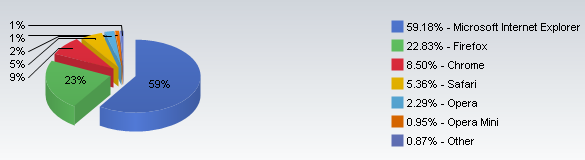
\includegraphics[height=3.5cm]{webbrowsers-share-2010-10}
% 
% \begin{flushright}
% Net Market Share Report, October 2010 \\
% {\small \url{http://www.netmarketshare.com/}}
% \end{flushright}
% \end{frame}

%%---------------------------------------------------------------------
\subsection{References}

%%---------------------------------------------------------------

\begin{frame}
\frametitle{References on linear models}

\begin{itemize}
 \item \small [Faraway, 2005] Faraway, J. (2005) Linear models with R. CRC Press.
 \item \small [Crawley, 2007] Crawley, M. J. The R book. Wiley.
 \item \small [Kutner et al., 2004] Kutner, M., Nachtsheim, C., Neter, J. and Li, W. (2004).
Applied Linear Statistical Models. McGraw-Hill.

 \end{itemize}
\end{frame}

%%---------------------------------------------------------------

\begin{frame}
\frametitle{Linear models with R}

\begin{itemize}
 \item \small [Faraway, 2002] Faraway, J. Practical Regression and Anova Using R.
 \url{http://cran.r-project.org/doc/contrib/Faraway-PRA.pdf}

 \item \small [Faraway, 2002] Faraway, J. Introduction to Probability and Statistics Using R.
 \url{http://www.lulu.com/items/volume_68/8123000/8123594/3/print/IPSUR.pdf}

 \end{itemize}
\end{frame}

%%---------------------------------------------------------------



\end{document}
